\documentclass[14pt, a4paper]{extarticle}
\usepackage{indentfirst}
\usepackage{titulpage}
\usepackage{listings}
\usepackage{color}

\textwidth 16cm
\textheight 25cm
\oddsidemargin -2.5mm
\evensidemargin -3mm
\topmargin -20mm
\parindent 1.25cm

\usepackage[unicode, pdftex]{hyperref}
\hypertarget{d6}{Определение инвариантного пространства}


\lstset{tabsize=2,
    breaklines,
    columns=fullflexible,
    flexiblecolumns,
    numbers=left,
    numberstyle={\footnotesize},
    extendedchars=\true
}
\lstdefinelanguage{MyC}{
  language=C,
  ndkeywordstyle=\color{darkgray}\bfseries,
  identifierstyle=\color{black},
  morecomment=[n]{/**}{*/},
  commentstyle=\color{blue}\ttfamily,
  stringstyle=\color{red}\ttfamily,
  morestring=[b]",
  showstringspaces=false,
  morecomment=[l][\color{gray}]{//},
  keepspaces=true,
  escapechar=\%,
  texcl=true
}

\begin{document}
    
    \fefutitlepage{Б9121-09.03.03пикд}{Яцевич К.А.}{2}{Февраля\hspace{30pt}}{23}
    \defaultfont
    
    \vspace{1cm}
   
    \pagebreak
   
    \tableofcontents
   
    \pagebreak

    \section*{Глоссарий}
    \addcontentsline{toc}{section}{Глоссарий}

    \textbf{Вершина(узел)} --- структурная единица графа

    \textbf{Ребро} --- соединяет вершины графа
    
    \textbf{Граф} --- математическая система, объекты которой обладают парными связями

    \textbf{Паросочетание} --- набор несмежных ребер

    \textbf{Свободная вершина} --- вершина графа, не покрытая паросочетанием

    \textbf{Не инцидентные ребра} --- отношение между рёбрами, в котором существует соединяющая их вершина.

    \textbf{Чередующаяся цепь} --- путь в графе, в котором для любых двух соседних рёбер верно, что одно из них принадлежит паросочетанию M, а другое нет.

    \textbf{Дополняющий(увеличивающий) путь} --- чередующаяся цепь, которая начинается и кончается свободными вершинами.

    \textbf{Цветок(соцветие/бутон)} --- нечетный цикл графа

    \textbf{Стебель} --- чередующаяся цепь чётной длины

    \textbf{База} --- вершина графа, которая пренадлежит стеблю и  является частю цикла

    \pagebreak
   
    \section*{Введение}
    \addcontentsline{toc}{section}{Введение}
   
    % \textit{Цель:} Научиться определять тип ДУ, пользоваться методом Эйлера, и с помощью программ компьютерной математики научиться решать представленные ниже задачи.\\
   
    % \subsection*{Постановка задачи}
    % Требуется разработать алгоритм  за ассимтотику $O(n^3)$. Провести тестирование с использованием ручных тестов и тестов с использованием генератора.
   
    \subsection*{Историческая справка}
    \addcontentsline{toc}{subsection}{Историческая справка}

    Алгоритмы поиска максимальных совпадений достаточно сложны. Джек Эдмондс сообщил о первом эффективном подходе в 1960-х годах, что стало важной вехой в истории компьютерных наук. Его <<Blossom algorithm>> вдохновил на вариации и альтернативы за последние несколько десятилетий.
    Эдмондс разработал алгоритм в 1961 году и опубликовал в 1965 году. 
    
    Основной причиной, почему алгоритм сжатия цветков важен, является то, что он дал первое доказательство возможности нахождения наибольшего паросочетания за полиномиальное время. 

    \pagebreak

    \section*{Постановка цели и задач работы}
    \addcontentsline{toc}{section}{Постановка цели и задач работы}

    \subsection*{Цель работы}
    \addcontentsline{toc}{subsection}{Цель работы}

    Изучить алгоритм "Сжатие цветков".

    \subsection*{Задачи работы}
    \addcontentsline{toc}{subsection}{Задачи работы}

    1. Изучить причины появления алгоритма, истрорию его создания.\\

    2. Изучить механику работы алгоритма, теоретическую часть.\\

    3. Реальзовать алгоритм.\\

    4. Продумаить тесты с наибольшим покрытием кода алгоритма.\\

    5. Провести тестирование алгоритма.\\

    6. Сделать выводы о проделанной работе.\\

    \pagebreak
    
    \section*{Описание алгоритма}
    \addcontentsline{toc}{section}{Описание алгоритма}

    \subsection*{Идея алгоритма}
    \addcontentsline{toc}{subsection}{Идея алгоритма}
    
    Алгоритм сжатия цветков (англ. Blossom algorithm) — это алгоритм в теории графов для построения наибольших паросочетаний на графах.
    
    Если дан граф $G=(V, E)$ общего вида, алгоритм находит паросочетание M такое, что каждая вершина из $V$ инцидентна не более чем одному ребру из $M$ и $|M|$ максимально. Паросочетание строится путем итеративного улучшения начального пустого паросочетания вдоль увеличивающих путей графа. 
    
    В отличие от двудольного паросочетания ключевой новой идеей было сжатие нечетного цикла в графе (цветка) в одну вершину с продолжением поиска итеративно по сжатому графу.

    \subsection*{Оценка сложности}
    \addcontentsline{toc}{subsection}{Оценка сложности}
    
    Пусть $n$ --- общее количество вершин, $n_1$ --- количество цветков,$n_2$ --- количество вершин в цветке,$m$ --- количество ребер. 

    Всего имеется $n$ итераций, на каждой из которых выполняется обход в ширину за $O(m)$ кроме того, могут происходить операции сжатия цветков — их может быть $O(n_1)$. Сжатие соцветий работает за $O(n_2)$, стоит отметить $n_1 \equiv n_2$, то есть общая асимптотика алгоритма составит $O(n(m+n^2))=O(n^3)$.

    \subsection*{Нахождение дополняющего(увеличивающего) пути}
    \addcontentsline{toc}{subsection}{Нахождение дополняющего(увеличивающего) пути}

    Пусть зафиксировано некоторое паросочетание $M$. Тогда простая цепь $P = (v_1, v_2, \ldots, v_k)$ называется чередующейся цепью, если в ней рёбра по очереди принадлежат --- не принадлежат паросочетанию $M$. Чередующаяся цепь называется увеличивающей, если её первая и последняя вершины не принадлежат паросочетанию. Иными словами, простая цепь $P$ является увеличивающей тогда и только тогда, когда вершина $v_1 \not\in M$, ребро $(v_2,v_3) \in M$, ребро $(v_4,v_5) \in M$, ..., ребро $(v_{k-2},v_{k-1}) \in M$, и вершина $v_k \not\in M$.

    Мы сможем найти максимальное паросочитание путем инверсии дополняющего пути.

    Основная проблема заключается в том, как находить увеличивающий путь. Если в графе имеются циклы нечётной длины, то просто обход в глубину/ширину будет работать некорректно --- при попадании в цикл нечётной длины обход может пойти по циклу в неправильном направлении.

    \pagebreak

    \subsection*{Сжатие цветка}
    \addcontentsline{toc}{subsection}{Сжатие цветка}

    \textbf{Сжатие цветка} — это сжатие всего нечётного цикла в одну псевдо-вершину (соответственно, все рёбра, инцидентные вершинам этого цикла, становятся инцидентными псевдо-вершине).
    
    \subsection*{Теорема Эдмондса}
    \addcontentsline{toc}{subsection}{Теорема Эдмондса}

    Пусть граф $\overline G$ был получен из графа G сжатием одного цветка.
    Тогда в графе $\overline G$ существует увеличивающая цепь тогда и только тогда, когда существует увеличивающая цепь в $G$.

    \textit{Доказательство}. 
    
    Обозначим через B цикл цветка, и через $\overline B$ соответствующую сжатую вершину.
    Вначале заметим, что достаточно рассматривать случай, когда база цветка является свободной вершиной (не принадлежащей паросочетанию). Действительно, в противном случае в базе цветка оканчивается чередующийся путь чётной длины, начинающийся в свободной вершине. Начиная со свободной вершины, помечаем не инцидентные ребра. Мощность паросочетания не изменится, а база цветка станет свободной вершиной. Итак, при доказательстве можно считать, что база цветка является свободной вершиной.

    Пусть путь $P$ является увеличивающим в графе $G$. Если он не проходит через B, то тогда, очевидно, он будет увеличивающим и в графе $\overline G$. Пусть P проходит через B. Тогда можно считать, что путь P представляет собой некоторый путь $P_1$, не проходящий по вершинам B, плюс некоторый путь $P_2$, проходящий по вершинам B и, возможно, другим вершинам. Но тогда путь $P_1$ + $\overline B$ будет являться увеличивающим путём в графе $\overline G$, что и требовалось доказать.

    \pagebreak
    
    \subsection*{Общая схема алгоритма}

    \addcontentsline{toc}{subsection}{Общая схема алгоритма}


    $N$ --- количество вершин
    
    $i$ --- вершина

    \begin{figure}[h!]
        \centering
        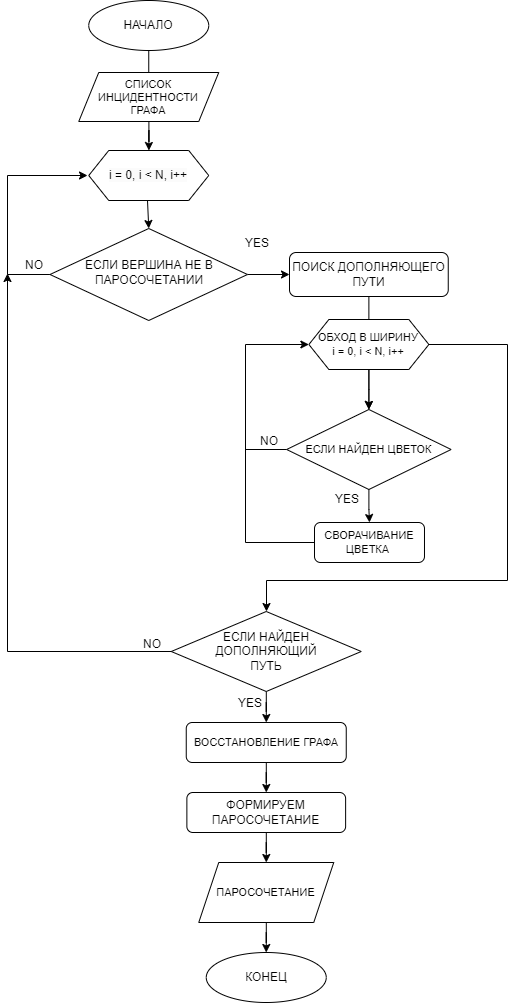
\includegraphics[scale=0.6]{block schema.png}
        \caption{Общая схема алгоритма}
        \label{fig:my_label}
    \end{figure}

    \pagebreak
    
    \subsection*{Пример работы алгоритма}
    \addcontentsline{toc}{subsection}{Пример работы алгоритма}


    \begin{figure}[h!]
        \centering
        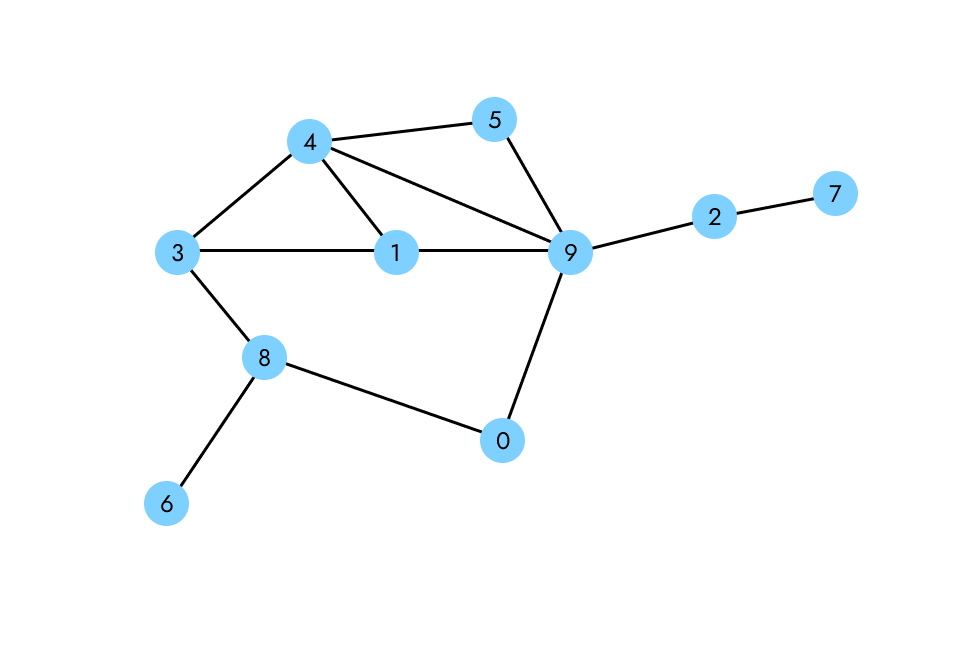
\includegraphics[scale=0.3]{1.png}
        \caption{Исходный граф}
        \label{fig:my_label}
    \end{figure}

    Начинаем рассматривать граф со свободной вершины 7. Двигаясь по ребрам обнаруживаем стебель: ребра 7-2 и  2-9. Следовательно, предполагаемый дополняющий путь будет начинаться со свободной вершины 7, ребро 2-9 --- паросочетание. Тогда вершина 9 является базой. С помощию BFS идем дальшне по графу:
    ребро 9-5, ребро 5-4, ребро 4-9 --- составляют нечетный цикл --- цветок.
    
    \begin{figure}[h!]
        \centering
        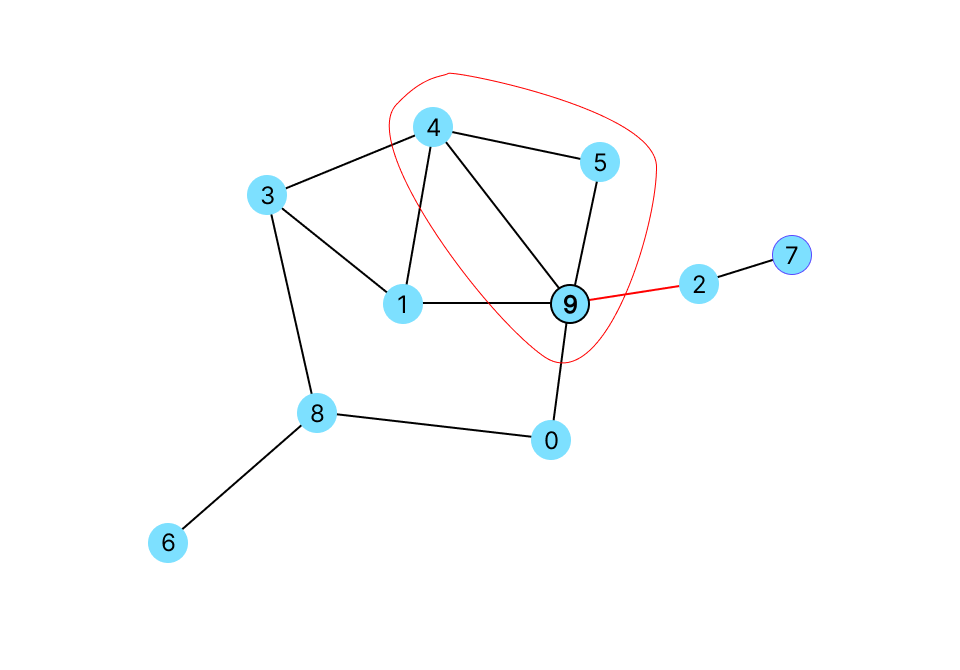
\includegraphics[scale=0.3]{2.png}
        \caption{Нахождение первого цветка}
        \label{fig:my_label}
    \end{figure}

    
    Вершины цикла сжимаем в базу. Получаем следующий граф, который продолжаем обрабатывать по тому же алгоритму.
    С помощию BFS идем дальше по графу:
    ребро 9-3, ребро 3-1, ребро 1-9 --- составляют нечетный цикл --- цветок.

    \begin{figure}[h!]
        \centering
        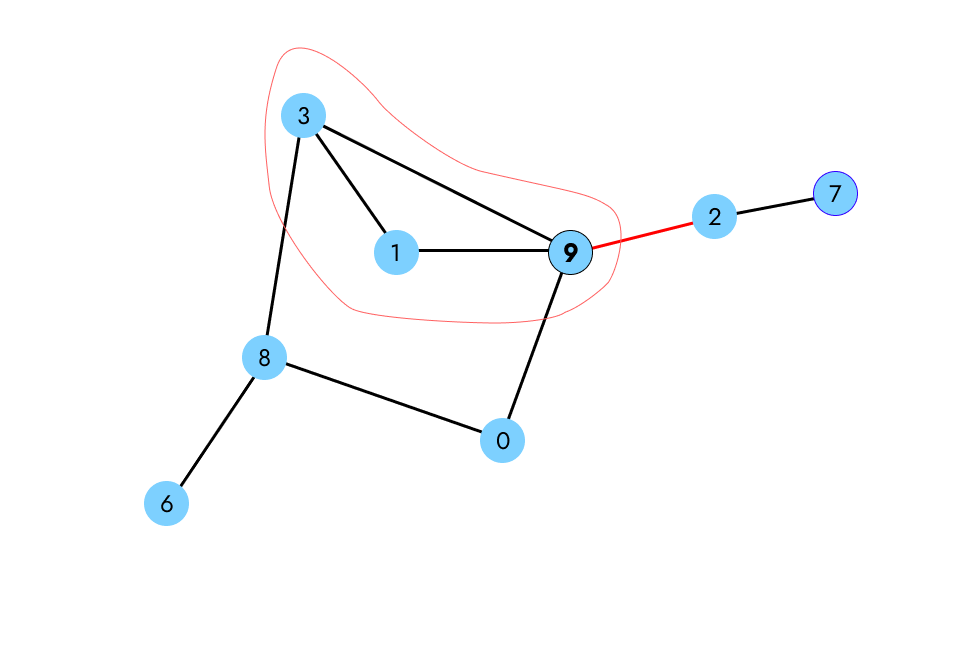
\includegraphics[scale=0.3]{3.png}
        \caption{Нахождение второго цветка}
        \label{fig:my_label}
    \end{figure} 

    \pagebreak

    Вершины цикла сжимаем в базу. Новый  граф снова обрабатываем.
    Ребра 9-8 8-0 и 0-9 --- составляют нечетный цикл --- цветок.

    \begin{figure}[h!]
        \centering
        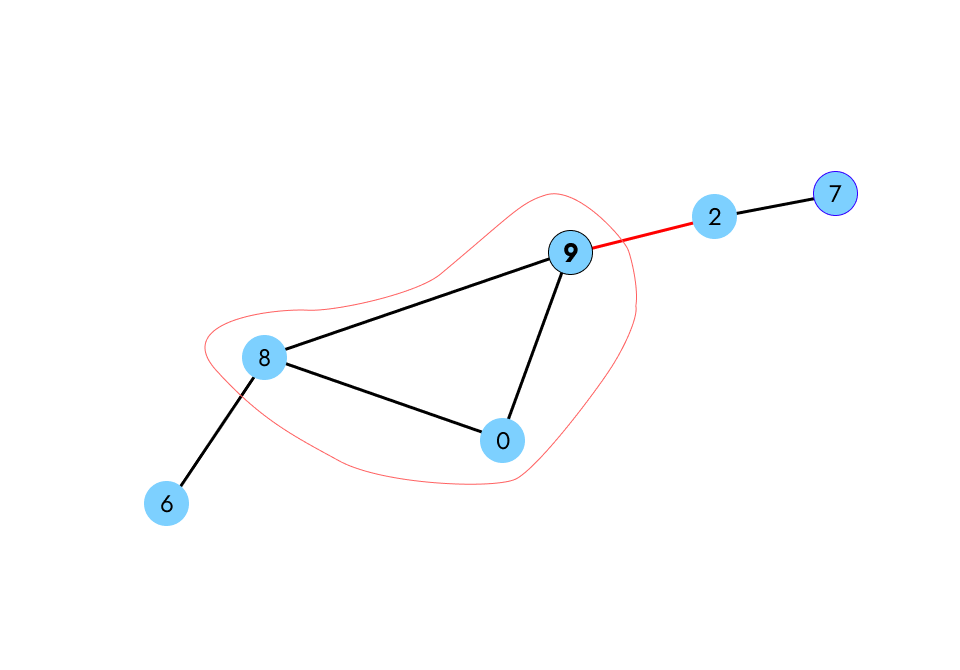
\includegraphics[scale=0.3]{4.png}
        \caption{Нахождение третьего цветка}
        \label{fig:my_label}
    \end{figure} 

    Сжимаем цветок и продолжаем анализировать граф. После базы 9 идет только одно ребро 9-6, окончание которого --- свободная вершина 6. Следовательно можем утверждать, что мы нашли дополняющий путь: 7-2, 2-9, 9-6.

    \begin{figure}[h!]
        \centering
        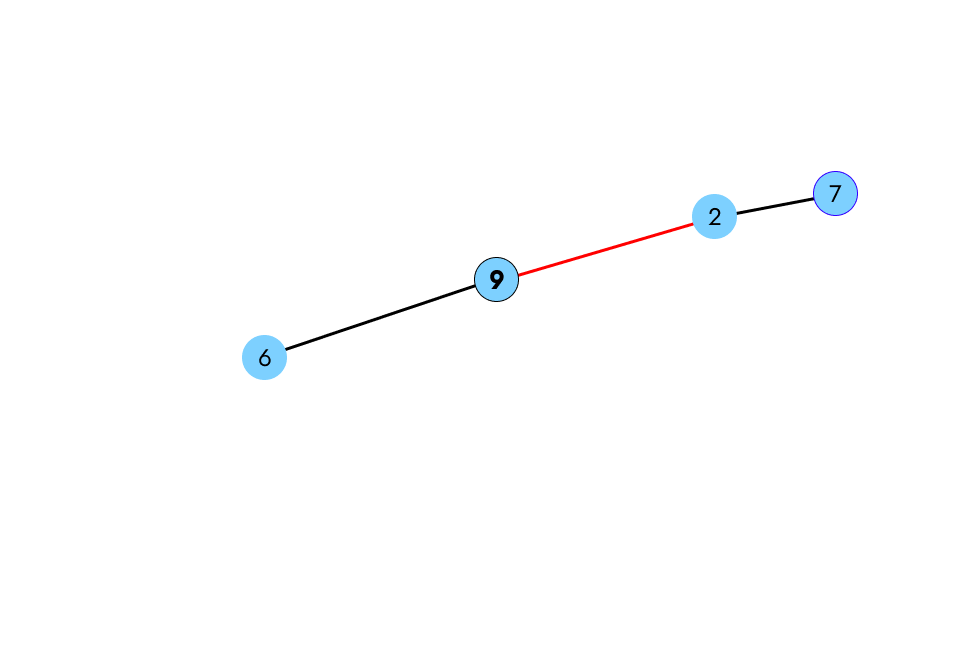
\includegraphics[scale=0.3]{5.png}
        \caption{Дополняющий путь}
        \label{fig:my_label}
    \end{figure} 

    \pagebreak

    Обращаемся к теореме Эдмондса:
    
    В графе $\overline G$ существует увеличивающая цепь тогда и только тогда, когда существует увеличивающая цепь в $G$.

    Значит мы можем приступить к восстановлению графа путем последовательного возвращения цветков.
    Для нахождения максимального паросочетания начнём с инверсии дополняющего пути.
    Начинаем восстановление с последнего сжатия цветка, инвертируя путь. При этом инвертрование пути подразумевает переопределение паросочетания. В цветке мы определяем паросочетание "в обратной последовательности": начиная с 9-0, переходя к 0-8. Так как в дополняющем пути база 9 была соединена с вершиной 6, то дойдя до узла, соединенного с вершиной 6, мы продолжаем переопределять паросочетание в направлении вершины 6.

    На данном этапе паросочетание составляет следующие не инцидентные ребра:
    7-2, 9-0, 8-6

    \pagebreak
    
    \begin{figure}[h!]
        \centering
        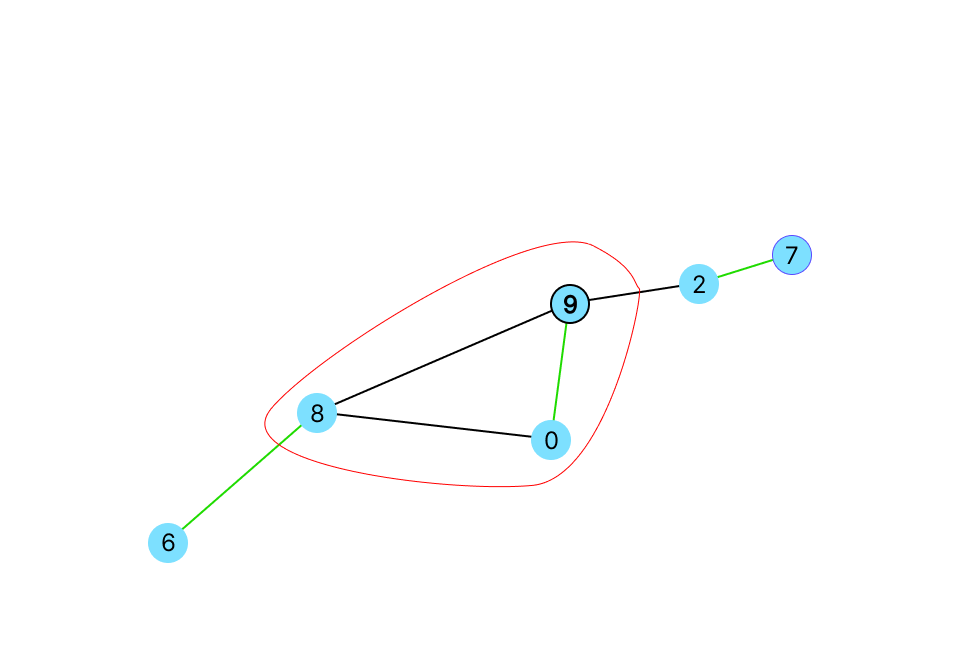
\includegraphics[scale=0.3]{6.png}
        \caption{Восстановление третьего цветка}
        \label{fig:my_label}
    \end{figure} 

    Запоминаем проставленное паросочетание и продолжаем восстановление графа. Ребро 7-2 уже инвертированно, поэтому переходим сразу к базе: в цветке определяем паросочетание "в обратной последовательности". База уже относится к ребру паросочетания, поэтому мы не можем пометить ребро 9-1. Значит помечаем следующее ребро 1-3. Аналогично с ребром 3-9.  

    На данном этапе паросочетание составляет следующие не инцидентные ребра:
    7-2, 9-0, 8-6, 3-1
    
    \begin{figure}[h!]
        \centering
        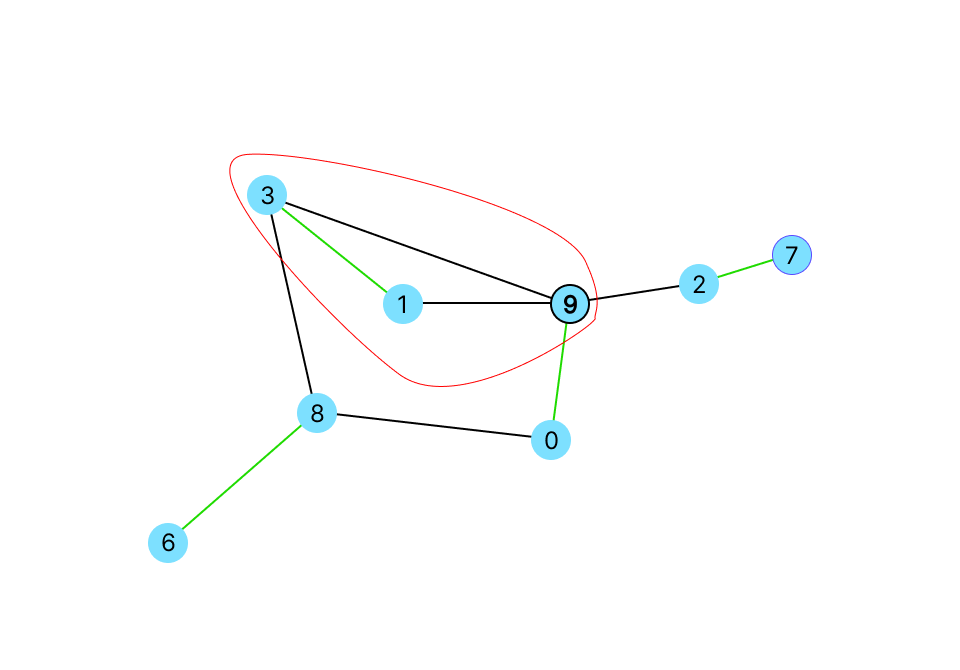
\includegraphics[scale=0.3]{8.png}
        \caption{Восстановление второго цветка}
        \label{fig:my_label}
    \end{figure} 

    \pagebreak

    Восстанавливаем последний цветок: аналогично помечаем ребра, начиная с базы. Ребро 9-4 --- не помечаем, ребро 4-5 --- помечаем, ребро 5-9 --- не помечаем. 

    \begin{figure}[ht!]
        \centering
        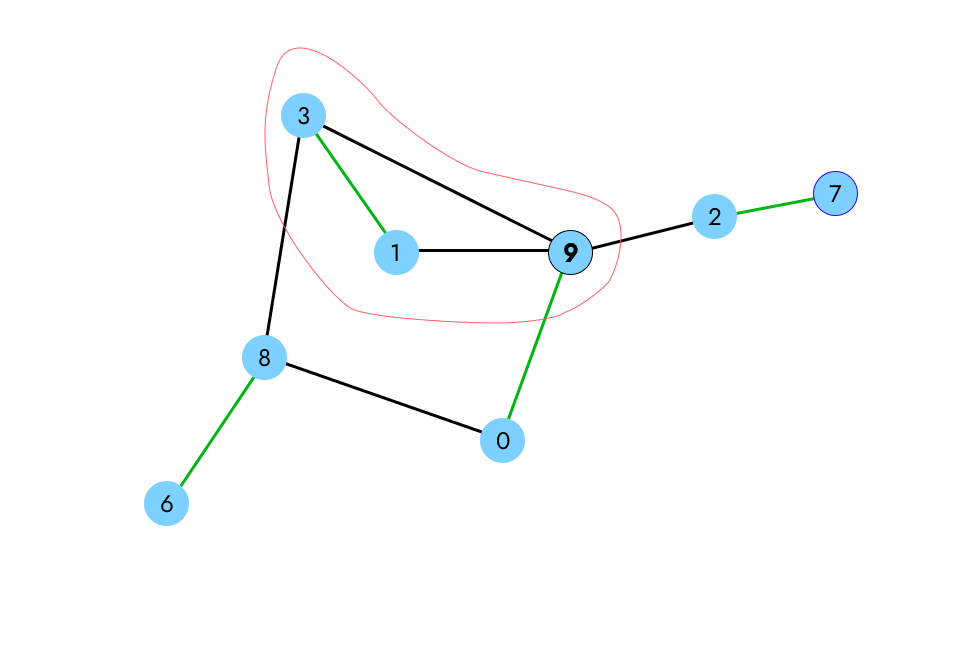
\includegraphics[scale=0.3]{7.png}
        \caption{Восстановление первого цветка}
        \label{fig:my_label}
    \end{figure} 

    Мы закончили восстановление графа и нашли максимальное паросочетание.

    \pagebreak
    
    \section*{Реализация}
    \addcontentsline{toc}{section}{Реализация}

    Для реализации алгоритма был выбран язык программирования С++, среда разработки --- Visual Studio 2022, является одним из самых популярных средств написания кода.
    Написана библиотека $blossom.h$ для нахождения максимального паросочетания, в которой реализованы следующие функции:

    \begin{lstlisting}[language=c++]
#pragma once
#include <vector>
#include <iostream>

int get_match(std::vector<std::vector<int>>&, std::vector<int>&);

void print_match(std::vector<int>&);
    \end{lstlisting}

    \subsection*{Поиск дополняющего пути}
    \addcontentsline{toc}{subsection}{Поиск дополняющего пути}

    Функция $get\_match()$ принимает список инцидентности и вектор, куда будет записано паросочетание. В результате работы помещает в переменную $a$ паросочетание.

    \begin{lstlisting}[language=c++]
int get_match(std::vector<std::vector<int>>& g, std::vector<int>& match) {

	match.clear();
	match.resize(g.size(), -1);
	std::vector<int> p;
	p.resize(g.size(), -1);

	for (int i = 0; i < g.size(); i++) {
		if (match[i] == -1) {
			int v = find_path(i, g, match, p);
			while (v != -1) {
				int pv = p[v], ppv = match[pv];
				match[v] = pv, match[pv] = v;
				v = ppv;
			}
		}
	}
	return 0;
}
    \end{lstlisting}

    \pagebreak

    Для реализации функции $get\_match()$ были написаны вспомогательные функции:\\

    Функция $lca()$ находит общего ближайшего предка для вершин цветка --- базу.

    \begin{lstlisting}[language=c++]
int lca(int a, int b, std::vector<int>& base, std::vector<int>& match, std::vector<int>& p) {
	std::vector<bool> used;
	used.resize(base.size(), false);
	for (;;) {
		a = base[a];
		used[a] = true;
		if (match[a] == -1)  break; // äîøëè äî êîðíÿ
		a = p[match[a]];
	}

	for (;;) {
		b = base[b];
		if (used[b])  return b;
		b = p[match[b]];
	}
}
    \end{lstlisting}

    Функция $mark\_path()$ помечает чередующийся путь. 

    \begin{lstlisting}[language=c++]
void mark_path(int v, int b, int children, std::vector<int>& base, std::vector<int>& match, std::vector<int>& p, std::vector<bool>& blossom) {
	while (base[v] != b) {
		blossom[base[v]] = blossom[base[match[v]]] = true;
		p[v] = children;
		children = match[v];
		v = p[match[v]];
	}
}

    \end{lstlisting}

    Функция $find\_path()$ ищет дополняющий путь из каждой вершины. Результатом работы функции является последняя вершина дополняющего пути.

    \begin{lstlisting}[language=c++]
int find_path(int root, std::vector<std::vector<int>> &g, std::vector<int> &match, std::vector<int>& p) {
	p.clear();
	p.resize(g.size(), -1);

	std::vector<bool> used;
	used.resize(g.size(), false);
	std::vector<bool> blossom;
	std::vector<int> q;
	q.resize(g.size(), 0);
	std::vector<int> base;

	for (int i = 0; i < g.size(); i++)
		base.push_back(i);

	used[root] = true;
	int qh = 0, qt = 0;
	q[qt++] = root;
	while (qh < qt) {
		int v = q[qh++];
		for (size_t i = 0; i < g[v].size(); i++) {
			int to = g[v][i];
			if (base[v] == base[to] || match[v] == to)  continue;
			if (to == root || match[to] != -1 && p[match[to]] != -1) {
				int curbase = lca(v, to, base, match, p);
				
				blossom.clear();
				blossom.resize(g.size(), false);

				mark_path(v, curbase, to, base, match, p, blossom);
				mark_path(to, curbase, v, base, match, p, blossom);
				for (int i = 0; i < g.size(); i++)
					if (blossom[base[i]]) {
						base[i] = curbase;
						if (!used[i]) {
							used[i] = true;
							q[qt++] = i;
						}
					}
			}
			else if (p[to] == -1) {
				p[to] = v;
				if (match[to] == -1)
					return to;
				to = match[to];
				used[to] = true;
				q[qt++] = to;
			}
		}
	}
	return -1;
}
    \end{lstlisting}

    Также была реализована функция $print\_match()$ --- принимает паросочетание и выводит его в консоль.

    \begin{lstlisting}[language=c++]
void print_match(std::vector<int>& a) {
	for (int i = 0; i < a.size(); i++) {
		if (i < a[i]) {
			std::cout << i << '-' << a[i] << "\n";
		}
	}
}
    \end{lstlisting}
    
    \pagebreak

    \section*{Тестирование}
    \addcontentsline{toc}{section}{Тестирование}

     Для проведения тестирования был создан набор из 37 файлов. Часть тестов были созданы вручную, остальные автомтатически сгенерированы на языке программирования $Python$.

    Реализация генератора

    \begin{lstlisting}[language=python]
import networkx as nx
import matplotlib.pyplot as plt
import scipy

n = vertices_count
constructor = [(n, n * n, 0.5)]
g = nx.random_shell_graph(constructor)
nx.draw(g, with_labels=True)
graph = [set() for _ in range(n)]
for i, j in g.edges():
    graph[j].add(i)
    graph[i].add(j)
    \end{lstlisting}

    Запись в файл в виде списка инцидентности:

    \begin{lstlisting}[language=python]
with open(r'C:\Users\user\source\repos\Blossom\graph.txt', 'w') as fout:
    for vertex in graph:
        print(*vertex, file=fout)
    \end{lstlisting}\\

    Тесты покрывают различные ситуации:

    Набор одиночных вершин; цепочек из ребер и вершин; некрупных (5-19 вершин), средних (20-100 вершин) и крупных (100+ вершин) произвольных графов с четным, нечетным стеблем и без него; некрупных (5-19 вершин), средних (20-100 вершин) и крупных (100+ вершин) полносвязных графов; лесов из разного количества деревьев разной сложности; произвольных графов, состоящих из более чем 100, 200 и 500.\\
    
    \pagebreak

    Каждый тест включает два файла: $input.txt$ и $output.txt$.
    Файл $input.txt$ сожержит список инцидентности: номер строки --- вершина; значения, записанные через пробел --- вершины, сопряженные с данной.\\

    Пример входного файла:

    \begin{lstlisting}[language=c++]
    3 4
    8 5
    3 6
    0 2 5 6 7 8
    0 6
    1 3 7
    2 3 4
    3 5
    1 3
    \end{lstlisting}    

    Файл $output.txt$ содержит только одно число --- количество несопряженных ребер в итоговом парасочетании.

    Проверка результатов работы программного кода осуществляется по критериям:\\

    1. Проверяется уникальность вершин в итоговом просочетании.\\

    2. Проверяется количество ребер в итоговом парасочетании относительно готового решения.\\

    3. Проверяется подлинность (существование) ребер в итоговом парасочетании.\\

    Данные критерии позволят исключить возможность упущения решений из возможного множества паросочетаний графа. Уникальность вершин позволит нам убедиться, что среди ребер нет смежных (в случае обнаручения неуникальной вершины, т.е. пренадрежащей двум ребрам, решение можно считать неверным). В случае, если граф имеет набор парасочетаний, то количество ребер в наборах будет всегда одинаковым. Ложное решение может соответствовать первым двум критериям, но содержать не подлинные ребра --- для этого необходимо проверить существование ребер в графе.
    \pagebreak

    \subsection*{Корректность алгоритма}
    \addcontentsline{toc}{subsection}{Корректность алгоритма}

    Проверка алгоритма на корректную работу проводилась следующим образом:

    Первый этап --- решение тестов вручную.

    Второй этап --- атоматическая проверка с помощью готового решения. 
    Для реализации второго этапа использовалась функция $networkx.max_weight_matching()$ из библиотеки $networkx$ языка программирования $Python$.

    Реализованный алгоритм и функция $networkx.max_weight_matching()$ возвращали одинаковый набор ребер на всех тестах.

    \subsection*{Производительность}
    \addcontentsline{toc}{subsection}{Производительность}

    Тестирование производительности проводилось на трех наборах графов: полносвязные графы, произвольные графи и лес. Тест производительности показал, что полносвязные графы больше всего нагружают алгоритм как по памяти, так и по времени работы.

    Вне зависимоти от структуры графа, время работы алгоритма не привышала 6 мс для графов до 100 вершин. При увеличении вершин наблюдаются различия в работе алгоритма:
    
    Работа алгоритма на полносвязных графах от 500 вершин больше по памяти (до 2 МБ) и дольше по времени (до 6.2 с).

    \begin{figure}[h!]
        \centering
        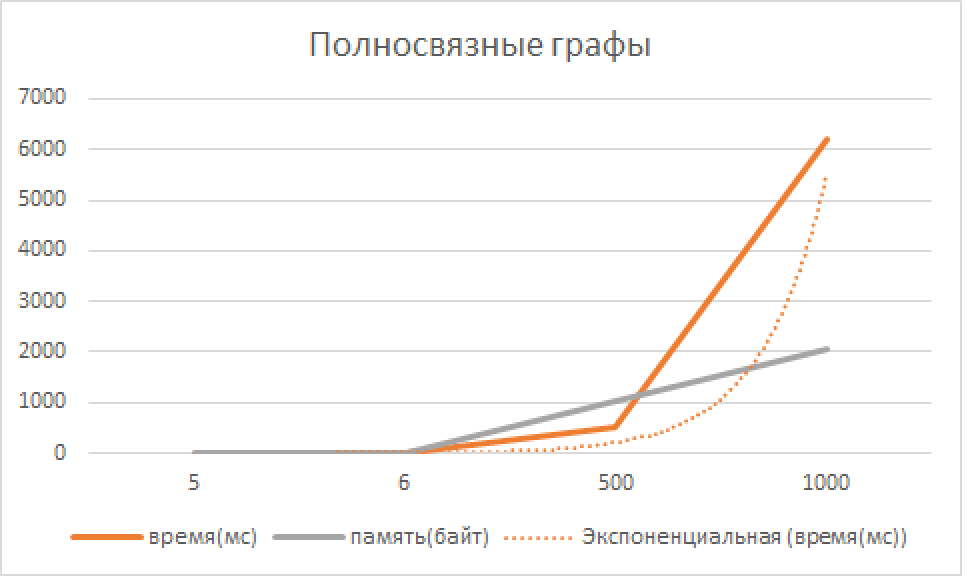
\includegraphics[scale=0.6]{fullyconnected_graphs.png}
        \caption{График зависимости памяти и времени от количества вершин для полносвязных графов}
        \label{fig:my_label}
    \end{figure} 

    Обработка произвольного графа от 100 вершин и более не занимает порядка 20 мс и не нагружает алгоритм по памяти.

    \pagebreak

    \begin{figure}[h!]
        \centering
        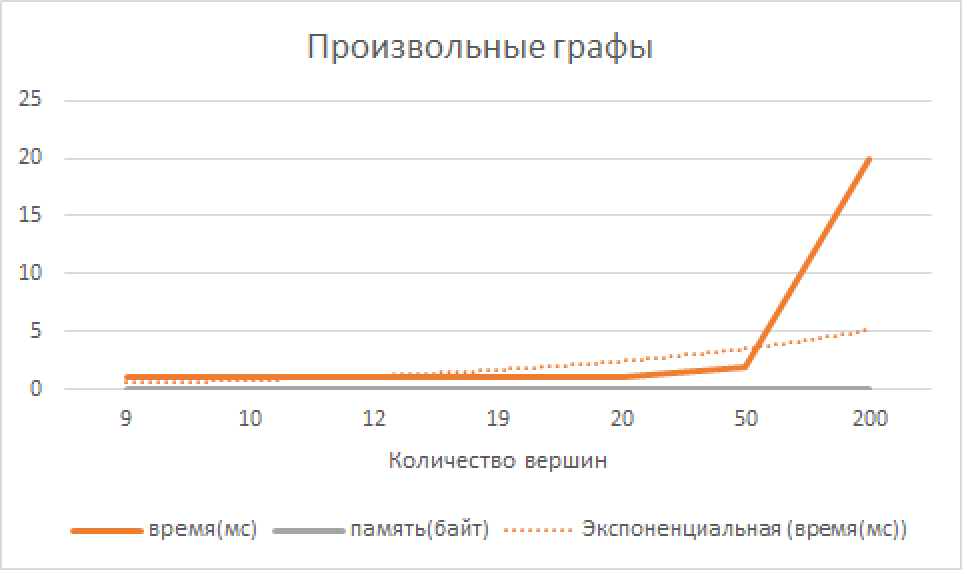
\includegraphics[scale=0.6]{arbitrary_graphs.png}
        \caption{График зависимости памяти и времени от количества вершин для произвольных графов}
        \label{fig:my_label}
    \end{figure}

    Результат отработки лесов свыше 100 вершин не нагружает память, но выходит дольше - от 6 мс и порядка 109 мс для 1000 вершин.

    \begin{figure}[h!]
        \centering
        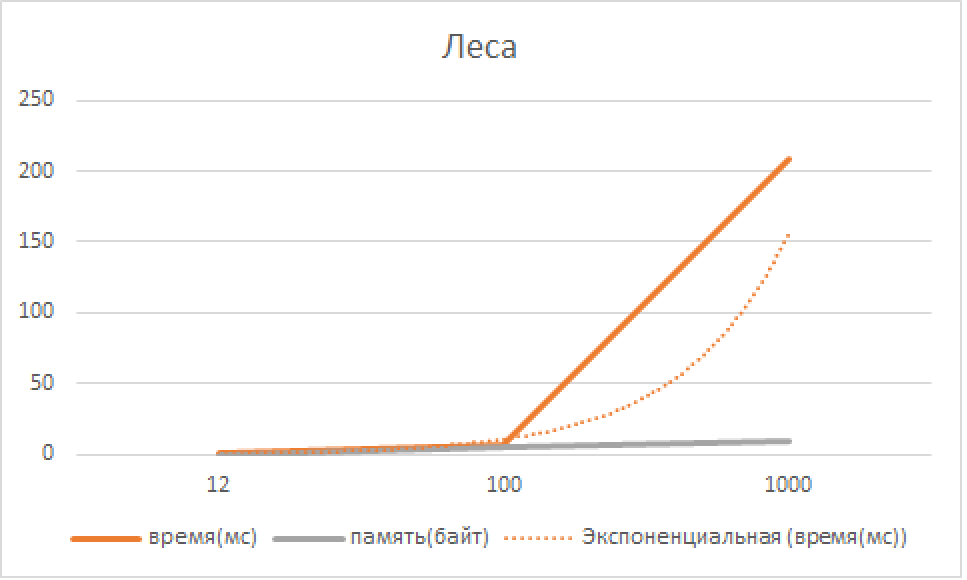
\includegraphics[scale=0.6]{forest.png}
        \caption{График зависимости памяти и времени от количества вершин для леса}
        \label{fig:my_label}
    \end{figure}    
    
    \pagebreak
    
    \subsection*{Результат теститрования производительности}
    \addcontentsline{toc}{subsection}{Результат теститрования производительности}

    По результатам тестирования было выявлено, что алгоритм работает корректно, было дрстигнуто 100\% покрытие кода.
    
    \begin{figure}[h!]
        \centering
        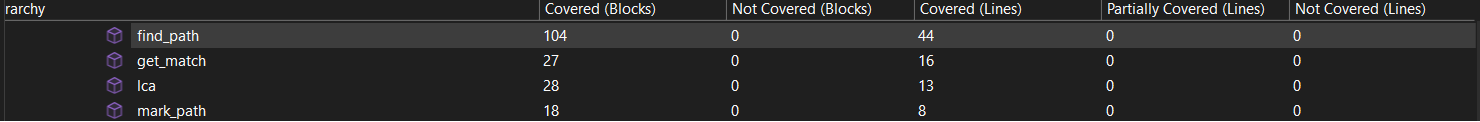
\includegraphics[scale=0.55]{coverage.png}
        \caption{Покрытие кода}
        \label{fig:my_label}
    \end{figure} 

    \section*{Сравнение}
    \addcontentsline{toc}{section}{Сравнение с алгоритмом Куна}

   Проведена сравнительная оценка с работой аналогичной функции для поиска максимального парасочетания --- $networkx.max_weight_matching()$ из библиотеки $networkx$ языка программирования $Python$.

   Время работы алгоритма и функции примерно одинаково на графах до 100, но алгоритм выигрывает по времени выполнения.
   
   Однако при большем количестве вершин на полносвязных графах функция работает значительно быстрее, чем реализованый алгоритм.

    \begin{figure}[h!]
        \centering
        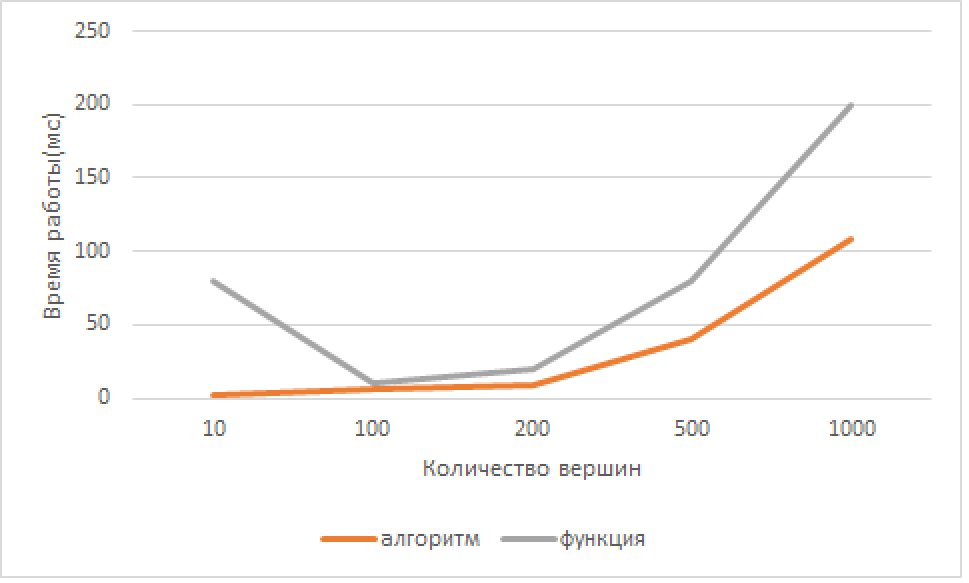
\includegraphics[scale=0.55]{comparison.png}
        \caption{График зависимости памяти и времени от количества вершин алгоритма и функции}
        \label{fig:my_label}
    \end{figure} 
   
    
    \pagebreak
    
    \section*{Заключение}
    \addcontentsline{toc}{section}{Заключение}

    В ходе изучения и реализации алгоритма были сделаны следующие выводы:

    1. Появление алгоритма «Сжатие цветков» позволило решать новые задачи на графах с нечетными циклами.\\
    
    2. Реализация библиотеки позволяет использовать алгоритм в других проектах.\\

    3. Тестирование показало, что алгоритм работает корректно и достаточно эффективно.\\

    4. Сравнительный анализ показал, что алгоритм работает эффективнее с малым количеством данных, но не сохраняет преимущество при больших объемах данных.\\

    \pagebreak
    
    \begin{thebibliography}{}

    \bibitem{1} 
    Jack Edmonds. Paths, trees, and flowers // Can. J. Math.. — 1965. — Т. 17. — С. 449–467.
    URL: \href{https://archive.org/details/sim_canadian-journal-of-mathematics_1965_17_3/page/448/mode/2up}{https://archive.org/details/sim\_canadian-journal-of-mathematics\_1965\_17\_3/page/448/mode/2up}\\
    
    \bibitem{2}
    Denth-First --- Edmonds' Blossom Algorithm Part 1: Cast of Characters. URL: \href{https://depth-first.com/articles/2020/09/28/edmonds-blossom-algorithm-part-1-cast-of-characters/}
    {https://depth-first.com/articles/2020/09/28/edmonds-blossom-algorithm-part-1-cast-of-characters/}\\

    \bibitem{3} 
    MAXimal --- Алгоритм Эдмондса нахождения наибольшего паросочетания в произвольных графах. 6 декабря 2012. 
    URL: \href{https://e-maxx.ru/algo/matching_edmonds}
    {https://e-maxx.ru/algo/matching\_edmonds}\\
    
    \bibitem{4}
    Энциклопедии Руниверсалис --- Алгоритм сжатия цветков.  28 ноября 2022. URL: \href{https://руни.рф/index.php/Алгоритм_сжатия_цветков#Цветки_и_стягивание}
    {https://руни.рф/index.php/Алгоритм\_сжатия\_цветков\#Цветки\_и\_стягивание}\\
    
    \bibitem{5}
    Единый центр по исследованию искусственного интеллекта "ЕЦИИИ" --- Алгоритм вырезания соцветий и сжатия цветков. URL: \href{https://intellect.icu/algoritm-vyrezaniya-sotsvetij-i-szhatiya-tsvetkov-8626}
    {https://руни.рф/index.php/Алгоритм\_сжатия\_цветков\#Цветки\_и\_стягивание}\\

    \bibitem{6}
    ИТМО, Викиконспекты --- Алгоритм вырезания соцветий.  4 сентября 2022. 
    URL: \href{https://neerc.ifmo.ru/wiki/index.php?title=Алгоритм_вырезания_соцветий}{https://neerc.ifmo.ru/wiki/index.php?title=Алгоритм\_вырезания\_соцветий}\\

    \bibitem{7}
    TUM. The Entrepreneurial University ---Edmonds's Blossom Algorithm. 2016 URL: \href{https://algorithms.discrete.ma.tum.de/graph-algorithms/matchings-blossom-algorithm/index_en.html}
    {https://algorithms.discrete.ma.tum.de/graph-algorithms/matchings-blossom-algorithm/index_en.html}\\

    \bibitem{8}
    Infogalactic: the planetary knowledge core --- Blossom algorithm. 19 February 2015. URL: \href{https://infogalactic.com/info/Blossom_algorithm}
    {https://infogalactic.com/info/Blossom_algorithm}\\

    \end{thebibliography}    
    
    \addcontentsline{toc}{section}{Список литературы}
    \printbibliography
    
\end{document}